\subsection{Neural Networks}
<<<<<<< Updated upstream
We performed unit tests of various functions of our fully-connected neural network (NN), convolutional neural network (CNN), and stochastic gradient descent (SGD) implementations to ensure their correctness.
Apart from this, the primary way we verified these implementations in a more integrated way was by testing toy network models on the MNIST database of handwritten digits\textcolor{blue}{\autocite{MNIST_Dataset}}.
After parsing the MNIST data into rust and creating data items for easy integration with our SGD trainer methods, we constructed toy NN and CNN models to train on this data.

Each MNIST input consisted of a $28 \times 28$ pixel image, and each output consisted of one of the ten labels $\{0, 1, \dots, 9\}$.
We therefore constructed the fully-connected NN to have 3 layers, with input and output sizes of $(784, 16)$, $(16, 16)$, and $(16, 10)$, respectively, thus taking the $28 \times 28 = 784$ pixels to one of two possible label probabilities.
For the CNN, we used the following layer structure: a convolutional layer with four $5 \times 5$ filters; a max pooling layer with a $2 \times 2$ window with stride $2$; a convolutional layer with two $5 \times 5 \times 4$ filters; another max pooling layer with a $2 \times 2$ window with stride $2$; and finally two fully-connected layers with input and output sizes of $(32, 16)$ and $(16, 10)$, respectively. Both convolutional layers had zero padding and stride $1$, and all the layers used a sigmoid activation function.

We trained these two networks using the MNIST data and the SGD trainer methods, with the learning rate set to $0.05$, a squared loss function, and a batch size of $32$.
The resulting accuracy after each epoch is shown in the plot below.

\begin{figure}[H]
  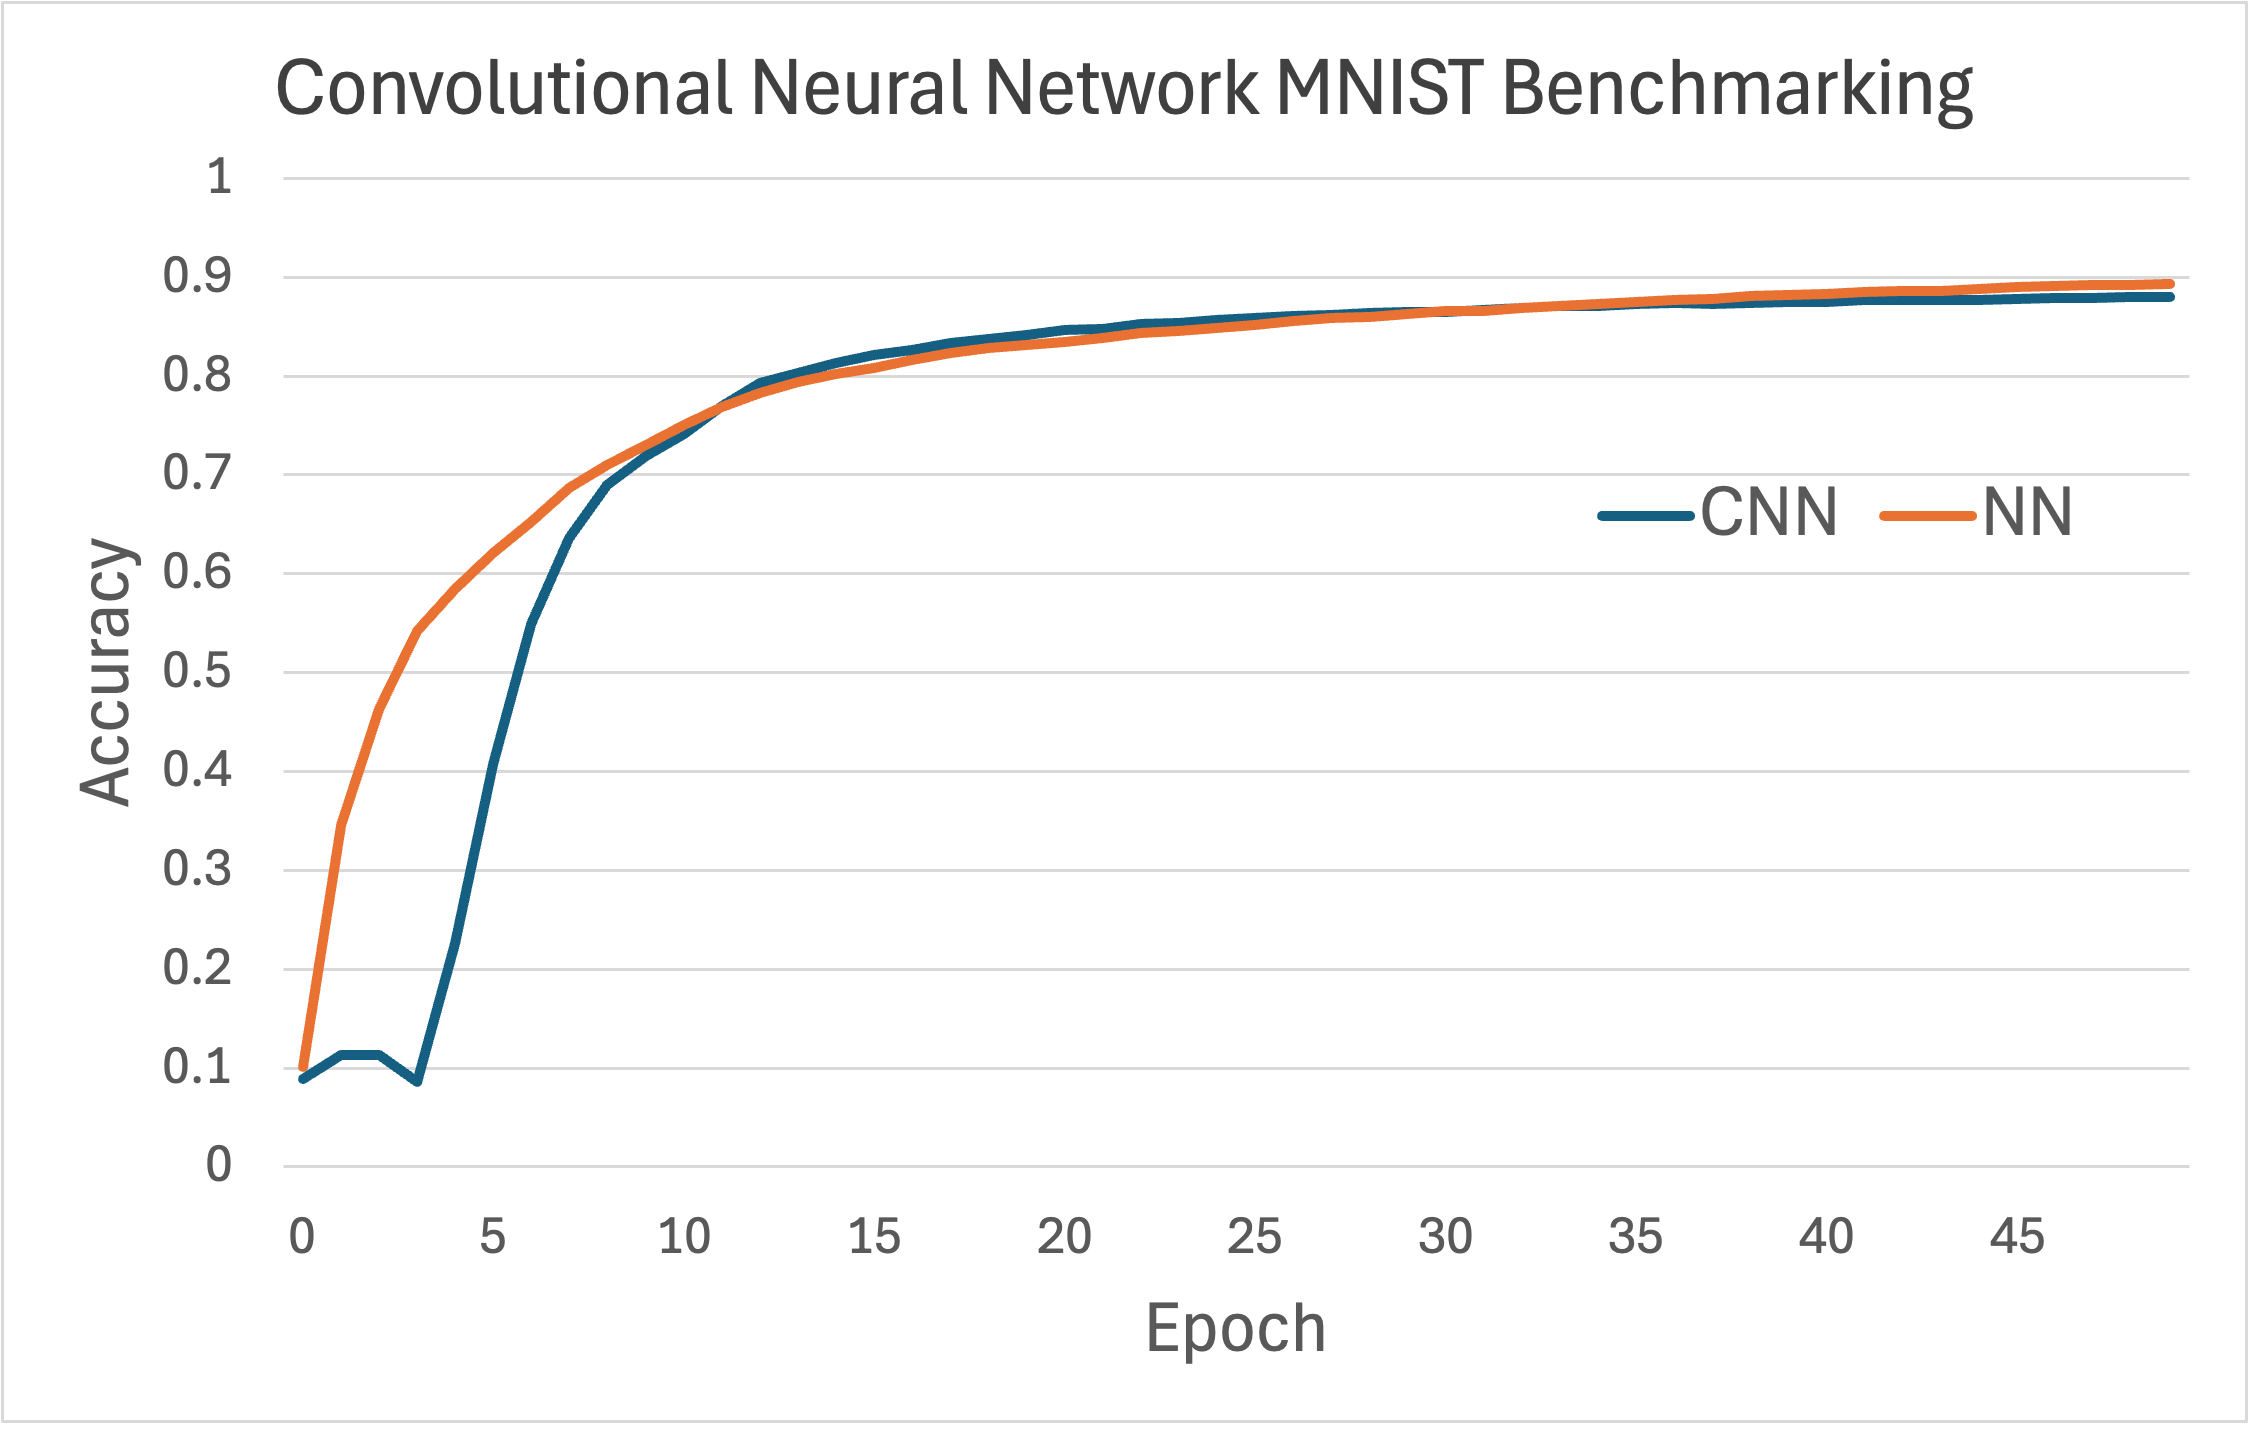
\includegraphics[width=\textwidth]{images/CNNBenchmarking.png}
\end{figure}

As can be seen, the two networks have a very similar performance curve, both achieving a classification accuracy of about $85\%$ after $20$ epochs, continuing more gradually up to $90\%$ by the $50$-th epoch.
Note that the CNN is specified by 1,004 total parameters while the fully-connected NN is specified by 13,002 total parameters.
Despite this, the two networks achieve a similar performance, demonstrating the advantage of the CNN.
However, it is important to note that the CNN took considerably longer to train for each epoch.
This is likely due to the overhead in the convolutional layers, stemming from some inefficient implementations in both CNN and matrix kit.

Regardless, this MNIST benchmarking shows that our implementations of NN, CNN, and SGD indeed yield trainable networks which can achieve good classification accuracies.
While not gauranteeing the correctness or efficiency of our implementations, this serves as a good integrated test to show that our implementations are behaving as intended.
